\documentclass[final]{beamer}

% Use beamerposter with A0 portrait
% \usepackage[size=a0,orientation=landscape,scale=1.05]{beamerposter}
\usepackage[size=a0,orientation=portrait,scale=1.05]{beamerposter}

% Basic packages
\usepackage[utf8]{inputenc}
\usepackage[T1]{fontenc}
\usepackage{lmodern}
\usepackage{graphicx}
\usepackage{booktabs}
\usepackage{multicol}
\usepackage{wrapfig}
\usepackage{natbib}
\bibliographystyle{unsrtnat}

% \usepackage{enumitem} % REMOVED to avoid beamer conflict
\usepackage{hyperref}
\usepackage{array}
\usepackage{ragged2e}
\usepackage{colortbl}
\usepackage{xcolor}
\usepackage{etoolbox} % for safe list tweaks
\usepackage{microtype}
\usepackage{tikz}
\usetikzlibrary{decorations.pathreplacing,calc}

% Safer list spacing
\makeatletter
\patchcmd{\itemize}{\def\makelabel}{\setlength{\itemsep}{0.4em}\def\makelabel}{}{}%
\patchcmd{\enumerate}{\def\makelabel}{\setlength{\itemsep}{0.4em}\def\makelabel}{}{}%
\makeatother

% Colors
\definecolor{royal}{HTML}{1D2A44}
\definecolor{accent}{HTML}{F18F01}
\definecolor{softbg}{HTML}{F4F1EB}
\definecolor{mint}{HTML}{2AA7A1}
\definecolor{violet}{HTML}{6C63FF}
\definecolor{danger}{HTML}{D1495B}

\setbeamercolor{normal text}{fg=royal,bg=softbg}
\setbeamercolor{structure}{fg=accent}
\setbeamercolor{alerted text}{fg=danger}
\setbeamercolor{block title}{fg=white,bg=royal}
\setbeamercolor{block body}{fg=royal,bg=white}
\setbeamercolor{block title alerted}{fg=white,bg=danger}
\setbeamercolor{block body alerted}{fg=royal,bg=white}
\setbeamercolor{titlewrap}{fg=white,bg=royal}
\setbeamercolor{titleaccent}{fg=accent,bg=royal}

\usefonttheme{professionalfonts}
\renewcommand{\familydefault}{\sfdefault}
\setbeamerfont{title}{series=\bfseries,family=\sffamily,shape=\upshape}
\setbeamerfont{block title}{series=\bfseries,family=\sffamily}
\setbeamerfont{block body}{family=\sffamily}
\setbeamerfont{section title}{series=\bfseries,family=\sffamily}
\setlength{\parskip}{0.65em}
\setlength{\parindent}{0pt}
\setlength{\columnsep}{1.8cm}
\setbeamertemplate{blocks}[rounded][shadow=true]
\newcommand{\key}[1]{\textbf{\color{accent}#1}}
\newcommand{\highlight}[1]{\textcolor{accent}{\textbf{#1}}}
\newcommand{\metriccard}[2]{%
  \begin{beamercolorbox}[wd=\linewidth,sep=0.75em,center,rounded=true,shadow=false]{block body}%
    {\Large\bfseries\color{accent}#1}\\[-0.25em]
    {\footnotesize #2}%
  \end{beamercolorbox}%
}
\newcommand{\callout}[2]{%
  \begin{beamercolorbox}[wd=\linewidth,sep=0.6em,rounded=true,shadow=false]{block body}%
    {\bfseries\color{royal}#1}\\[-0.3em]
    {\footnotesize #2}%
  \end{beamercolorbox}%
}

% Paper size
% \setlength{\paperwidth}{841mm}
% \setlength{\paperheight}{1189mm}

\setbeamertemplate{background}{%
  \begin{tikzpicture}[remember picture,overlay]
    \path[fill=softbg] (current page.south west) rectangle (current page.north east);
    \path[fill=accent!15!white] (current page.north west)
      .. controls +(12,0) and +(-8,-12) .. ($(current page.center)+(0,28)$)
      .. controls +(6,-12) and +(-12,-4) .. (current page.north west);
    \path[fill=violet!12!white] (current page.south east)
      .. controls +(-12,3) and +(6,12) .. ($(current page.center)+(0,-32)$)
      .. controls +(-6,10) and +(10,-3) .. (current page.south east);
    \path[fill=mint!10!white] ($(current page.center)+(0,36)$) circle (38cm);
  \end{tikzpicture}%
}

\title{\textbf{Refining the Sunspot Number Series to ISN~V3}}
\subtitle{Challenges and Benefits for the Space Climate Community}
\author{\large Kalugodu Chandrashekhar$^{1}$, Laure Lef\`evre$^{1}$, Benjamin Mampaey$^{1}$, Senthamizh Pavai Valliappan$^{1}$, Hisashi Hayakawa$^{2}$, Christian Ritter$^{3}$}
\institute{\small $^{1}$ Royal Observatory of Belgium (ROB), $^{2}$ Nagoya University, $^{3}$ Universit\'e Catholique de Louvain, Louvain-la-Neuve, Belgium}

% Logos (replace with your own files)
\newcommand{\leftlogo}{./logos/observatory_400x332.jpg}
\newcommand{\rightlogo}{./logos/BELSPO_1867x1563.jpg}

% Title box
\setbeamertemplate{headline}{%
  \leavevmode
  \begin{tikzpicture}[remember picture,overlay]
    \path[fill=royal] (current page.north west) rectangle ($(current page.north east)+(0,-6.1cm)$);
    \path[fill=accent!45!royal] ($(current page.north west)+(0,-0.2cm)$)
      .. controls +(8,-1) and +(-4,4) .. ($(current page.north)+(0,-3cm)$)
      .. controls +(4,-3) and +(-6,1) .. ($(current page.north west)+(0,-6.1cm)$);
    \path[fill=mint!45!royal,opacity=0.65] ($(current page.north east)+(-4cm,-0.5cm)$) circle (4.6cm);
  \end{tikzpicture}%
  \begin{beamercolorbox}[wd=\paperwidth,ht=10.8cm,dp=0ex,leftskip=2.2cm,rightskip=2.2cm]{titlewrap}
    \begin{minipage}[c]{0.17\paperwidth}
      \centering \vspace{-6.2cm}
      \includegraphics[height=4.9cm]{\leftlogo}
    \end{minipage}%
    \begin{minipage}[c]{0.51\paperwidth}
      \raggedright \vspace{-7.5cm}
%      {\fontsize{60}{62}\selectfont \textbf{FAR\textcolor{accent}{Su}N}}\\[-0.1cm]
%      {\small \color{accent}\textbf{Findability and Accessibility of historical Raw Sunspot Numbers}}\\[0.25cm]
      {\color{white}\bfseries\fontsize{40}{42}\selectfont \inserttitle}\\[0.4cm]
      {\color{accent!15!white}\fontsize{26}{28}\selectfont \insertsubtitle}\\[0.55cm]
      {\color{white}\normalsize \insertauthor}\\[0.25cm]
      {\color{softbg!70!white}\small \insertinstitute}
    \end{minipage}%
    \begin{minipage}[c]{0.22\paperwidth}
      \raggedleft \vspace{-6.2cm}
      \includegraphics[height=4.9cm]{\rightlogo}\\[0.5cm]
%      \callout{ISN heritage}{1607--1980 primary sources}\\[0.4cm]
%      \callout{Release goal}{ISN V3 with open uncertainties}
    \end{minipage}
  \end{beamercolorbox}%
  \vspace{0.8cm}
}

% Footer
\setbeamertemplate{footline}{%
  \begin{tikzpicture}[remember picture,overlay]
    \path[fill=royal!92!black] (current page.south west) rectangle ($(current page.south east)+(0,1.5cm)$);
    \path[fill=accent!55!royal] ($(current page.south west)+(0,0.15cm)$)
      -- ($(current page.south east)+(-5cm,0.15cm)$)
      .. controls +(-3,0.6) and +(4,-0.6) .. ($(current page.south west)+(6cm,1.5cm)$)
      -- cycle;
  \end{tikzpicture}%
  \begin{beamercolorbox}[wd=\paperwidth,ht=1.3cm,dp=0ex,leftskip=2.2cm,rightskip=2.2cm]{titlewrap}
    \vspace{0.2cm}
    \small
    \textbf{Contact}\,\,: \href{mailto:silso.info@observatory.be}{silso.info@observatory.be}\hfill
    \textbf{Data Portal}: \url{https://www.sidc.be/silso/}\hfill
    \textbf{Version}: Early 2025 snapshot
  \end{beamercolorbox}%
}

% Helper block env
\newenvironment{tightblock}[1]{%
  \begin{block}{#1}\vspace{0.35em}
}{\end{block}}

\begin{document}
\begin{frame}[t]
\begin{columns}[t,totalwidth=0.98\paperwidth]

% -------- COLUMN 1 --------
\begin{column}{0.27\paperwidth}
\begin{tightblock}{Abstract}
\justifying
The International Sunspot Number (ISN) remains affected by historical scale jumps such as the \emph{Waldmeier break}, even after two major recalibrations. FARSuN (Findability and Accessibility of historical Raw Sunspot Numbers) tackles this by rebuilding the record from the ground up: collecting handwritten logs and tables from 1607--1980, digitizing them, and applying consistent metadata and validation. 
  % Early 2025 milestones include integrating the full 1610--1918 \emph{Mittheilungen} corpus, digitizing more than 95\% of the 2\,000+ Zürich observation tables, extracting 338 drawings (1\,056 entries) from the C.\,H. Adams notebooks, and launching quality-control pipelines for the Gruithuisen manuscripts. The reconstructed ISN~V3 will deliver traceable uncertainties, hemispheric indices, and open FAIR-compliant access, strengthening space climate studies, solar cycle prediction, and coupled Sun--Earth research.
\end{tightblock}

\begin{tightblock}{Project Pulse}
\begin{minipage}[t]{0.48\linewidth}
  \metriccard{1607--1980}{Temporal coverage of raw records}
\end{minipage}\hfill
\begin{minipage}[t]{0.48\linewidth}
  \metriccard{2\,000+}{Zürich observation tables tracked}
\end{minipage}\\[0.6em]
\begin{minipage}[t]{0.48\linewidth}
  \metriccard{1\,056}{C. H. Adams notebook entries curated}
\end{minipage}\hfill
\begin{minipage}[t]{0.48\linewidth}
  \metriccard{100\%}{Wolf's \emph{Mittheilungen} corpus integrated}
\end{minipage}
\end{tightblock}

\begin{tightblock}{Why Reconstruction?}
  The ISN inherits observer-dependent scale changes (for example the 1947 "Waldmeier jump") that cannot be removed by tweaking coefficients alone. FARSuN pioneers a full reconstruction that replays the entire observing chain.
\begin{itemize}
  \item \textbf{Recalibration} only rescales an existing index; legacy gaps, missing metadata, and hidden assumptions stay baked in.
  \item \textbf{Reconstruction} retrieves the primary artefacts (drawings, tabular logs, weather notes) and recomputes the index with transparent uncertainty tracking.
  \item Direct access to the raw sources lets us audit outliers, model observer response curves, and issue reproducible releases such as ISN~V3.
\end{itemize}
\end{tightblock}

% \begin{tightblock}{Recalibration vs Reconstruction}
% \begin{minipage}[t]{0.48\linewidth}
%   \callout{Legacy recalibration}{Linear scaling of composite series; no new metadata; residual biases (e.g. "Waldmeier jump") remain hidden.}
% \end{minipage}\hfill
% \begin{minipage}[t]{0.48\linewidth}
%   \callout{FARSuN reconstruction}{Primary sources re-digitised with observer context, transparent uncertainty budgets, and reproducible release tooling.}
% \end{minipage}
% \vspace{0.3cm}
% {\scriptsize Based on FARSuN interactive report section "The Problem" \& "The Solution".}
% \end{tightblock}

\begin{tightblock}{How Reconstruction Works: Four-Axis Methodology}
\begin{enumerate}
  \item \key{Gather Sources}: track down dispersed observing logs (Wolf's \emph{Mittheilungen}, Zürich tables, Gruithuisen manuscripts, Adams drawings) and capture provenance metadata at ingest.
  \item \key{Process Data}: use handwriting/OCR engines (Transkribus models, custom scripts) alongside manual double-keying for fragile entries.
  \item \key{Validate \& Standardize}: reconcile aliases, observer IDs, and calendars; model group/spot counting behaviour to derive calibration curves.
  \item \key{Disseminate}: publish machine-readable products, APIs, and VO-ready services with versioned uncertainty bundles for each release.
\end{enumerate}
\end{tightblock}

\begin{tightblock}{FAIR Principles}
  Every dataset and release roadmap is benchmarked against FAIR targets that we monitor with the dashboard shown below.

\begin{itemize}
  \item \textbf{Findable} – persistent DOIs, rich observation-level metadata, and navigable catalogues.
  \item \textbf{Accessible} – open formats (CSV, NetCDF, VO tables) served via HTTPS and scripted download recipes.
  \item \textbf{Interoperable} – shared vocabularies, observer IDs, and VOEvent-ready semantics.
  \item \textbf{Reusable} – versioned releases with uncertainty models, provenance trails, and detailed caveats.
\end{itemize}
% 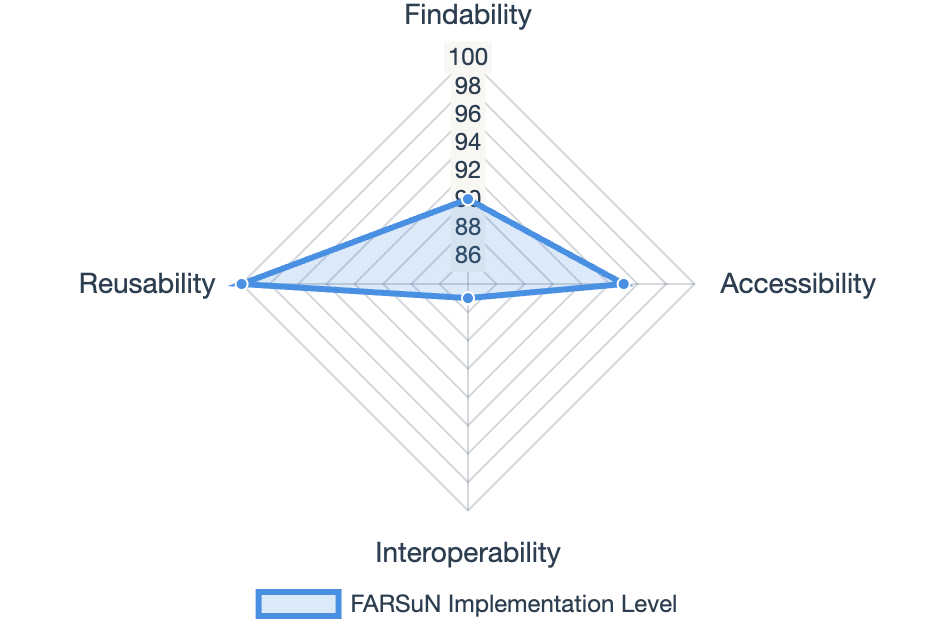
\includegraphics[width=\linewidth]{./figures/fair_radar.png}
\end{tightblock}
\begin{tightblock}{FARSuN Historical Sunspot Database — Status \& Outlook}
  \textbf{Present Status}
  \begin{itemize}
    \item Legacy sources (Mitteilungen, Wolf Institute, Shreya, Stephen, etc.) have been integrated into the current schema for cross-validation and QC.
    \item Automated quality checks detect inconsistencies (e.g., NG $>$ NS, duplicates, missing metadata).
    \item Metadata harmonization for observers, instruments, and observatories is underway, aligned with the EPN-TAP/VO standard for public access.
    \item A TAP server at ROB is operational, enabling ADQL queries and VOTable outputs.
  \end{itemize}

  \textbf{Next Steps}
  \begin{itemize}
    \item Finalize canonical schema and close remaining legacy mappings.
    \item Expand automated QC dashboards and uncertainty modeling.
    \item Scale up digitization and extraction (Adams, Gruithuisen, Herschel, etc.) using HTR and citizen-science workflows.
    \item Expose the full dataset through the EPN-TAP service, ensuring FAIR data availability.
    \item Use this harmonized database as the foundation for ISN V3 calibration and long-term solar activity studies.
  \end{itemize}

  \textbf{Goal}\\
  A sustainable, interoperable reference database ensuring that four centuries of solar observations remain accessible and scientifically reliable for the next generation of Sun-climate research.
\end{tightblock}
\end{column}


% -------- COLUMN 2 --------
\begin{column}{0.42\paperwidth}
\begin{tightblock}{Key Datasets}
\textbf{Mittheilungen Dataset — Present Status and Future}\\
The Mittheilungen journals, compiled by Rudolf Wolf and successors at the Zürich Observatory, form the backbone of historical sunspot observations, recording daily group and spot counts from 1848 to 1945 and extending back to 1610 through Wolf's compilations; within the FARSuN project, the complete series was digitized and structured (2017--2019) at the Royal Observatory of Belgium, integrated into the historical sunspot database, and is undergoing continuing quality checks, metadata harmonization, and cross-comparisons with new extractions.

\textbf{Current focus}
\begin{itemize}
  \item Refining data consistency and observer calibration (Wolf--Wolfer overlap).
  \item Finalizing metadata alignment for FAIR publication (EPN-TAP/VO-TAP).
  \item Resolving remaining ID and provenance issues across merged databases.
\end{itemize}

\textbf{Next steps}
\begin{itemize}
  \item Full public release via Virtual Observatory access.
  \item Inclusion of Mittheilungen as the core calibration reference for ISN Version 3.
  \item Development of interactive QC dashboards and documentation to support open, traceable historical solar research.
\end{itemize}
\begin{figure}[t]
  \centering
  \begin{minipage}[t]{0.4\linewidth}
    \centering
    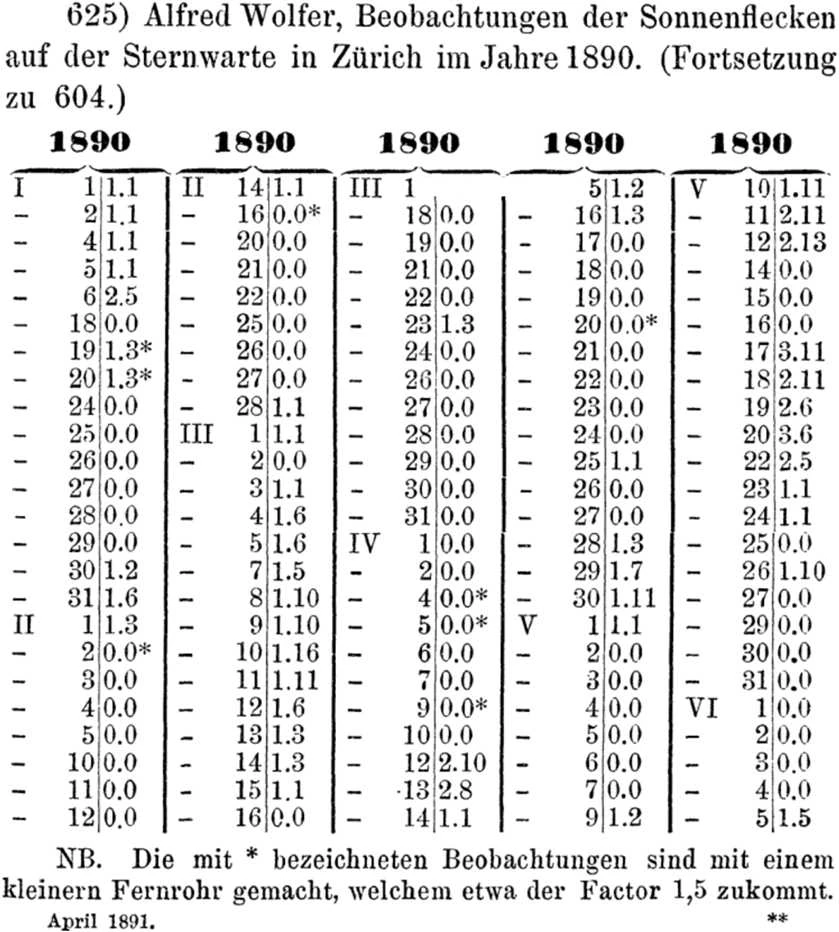
\includegraphics[width=\linewidth]{./figures/mittheilungen_sample.png}
    {\small (a) Facsimile of a typical yearly table, as published in the \textit{Mitteilungen}}
    % {(first page going up to early June). The table lists all daily observations from A.~Wolfer for 1890 with group and spot totals separated by a dot; stars mark days observed with a 40\,mm ``Parisian'' telescope.}
  \end{minipage}
  \hfill
  \begin{minipage}[t]{0.52\linewidth}
    \centering
    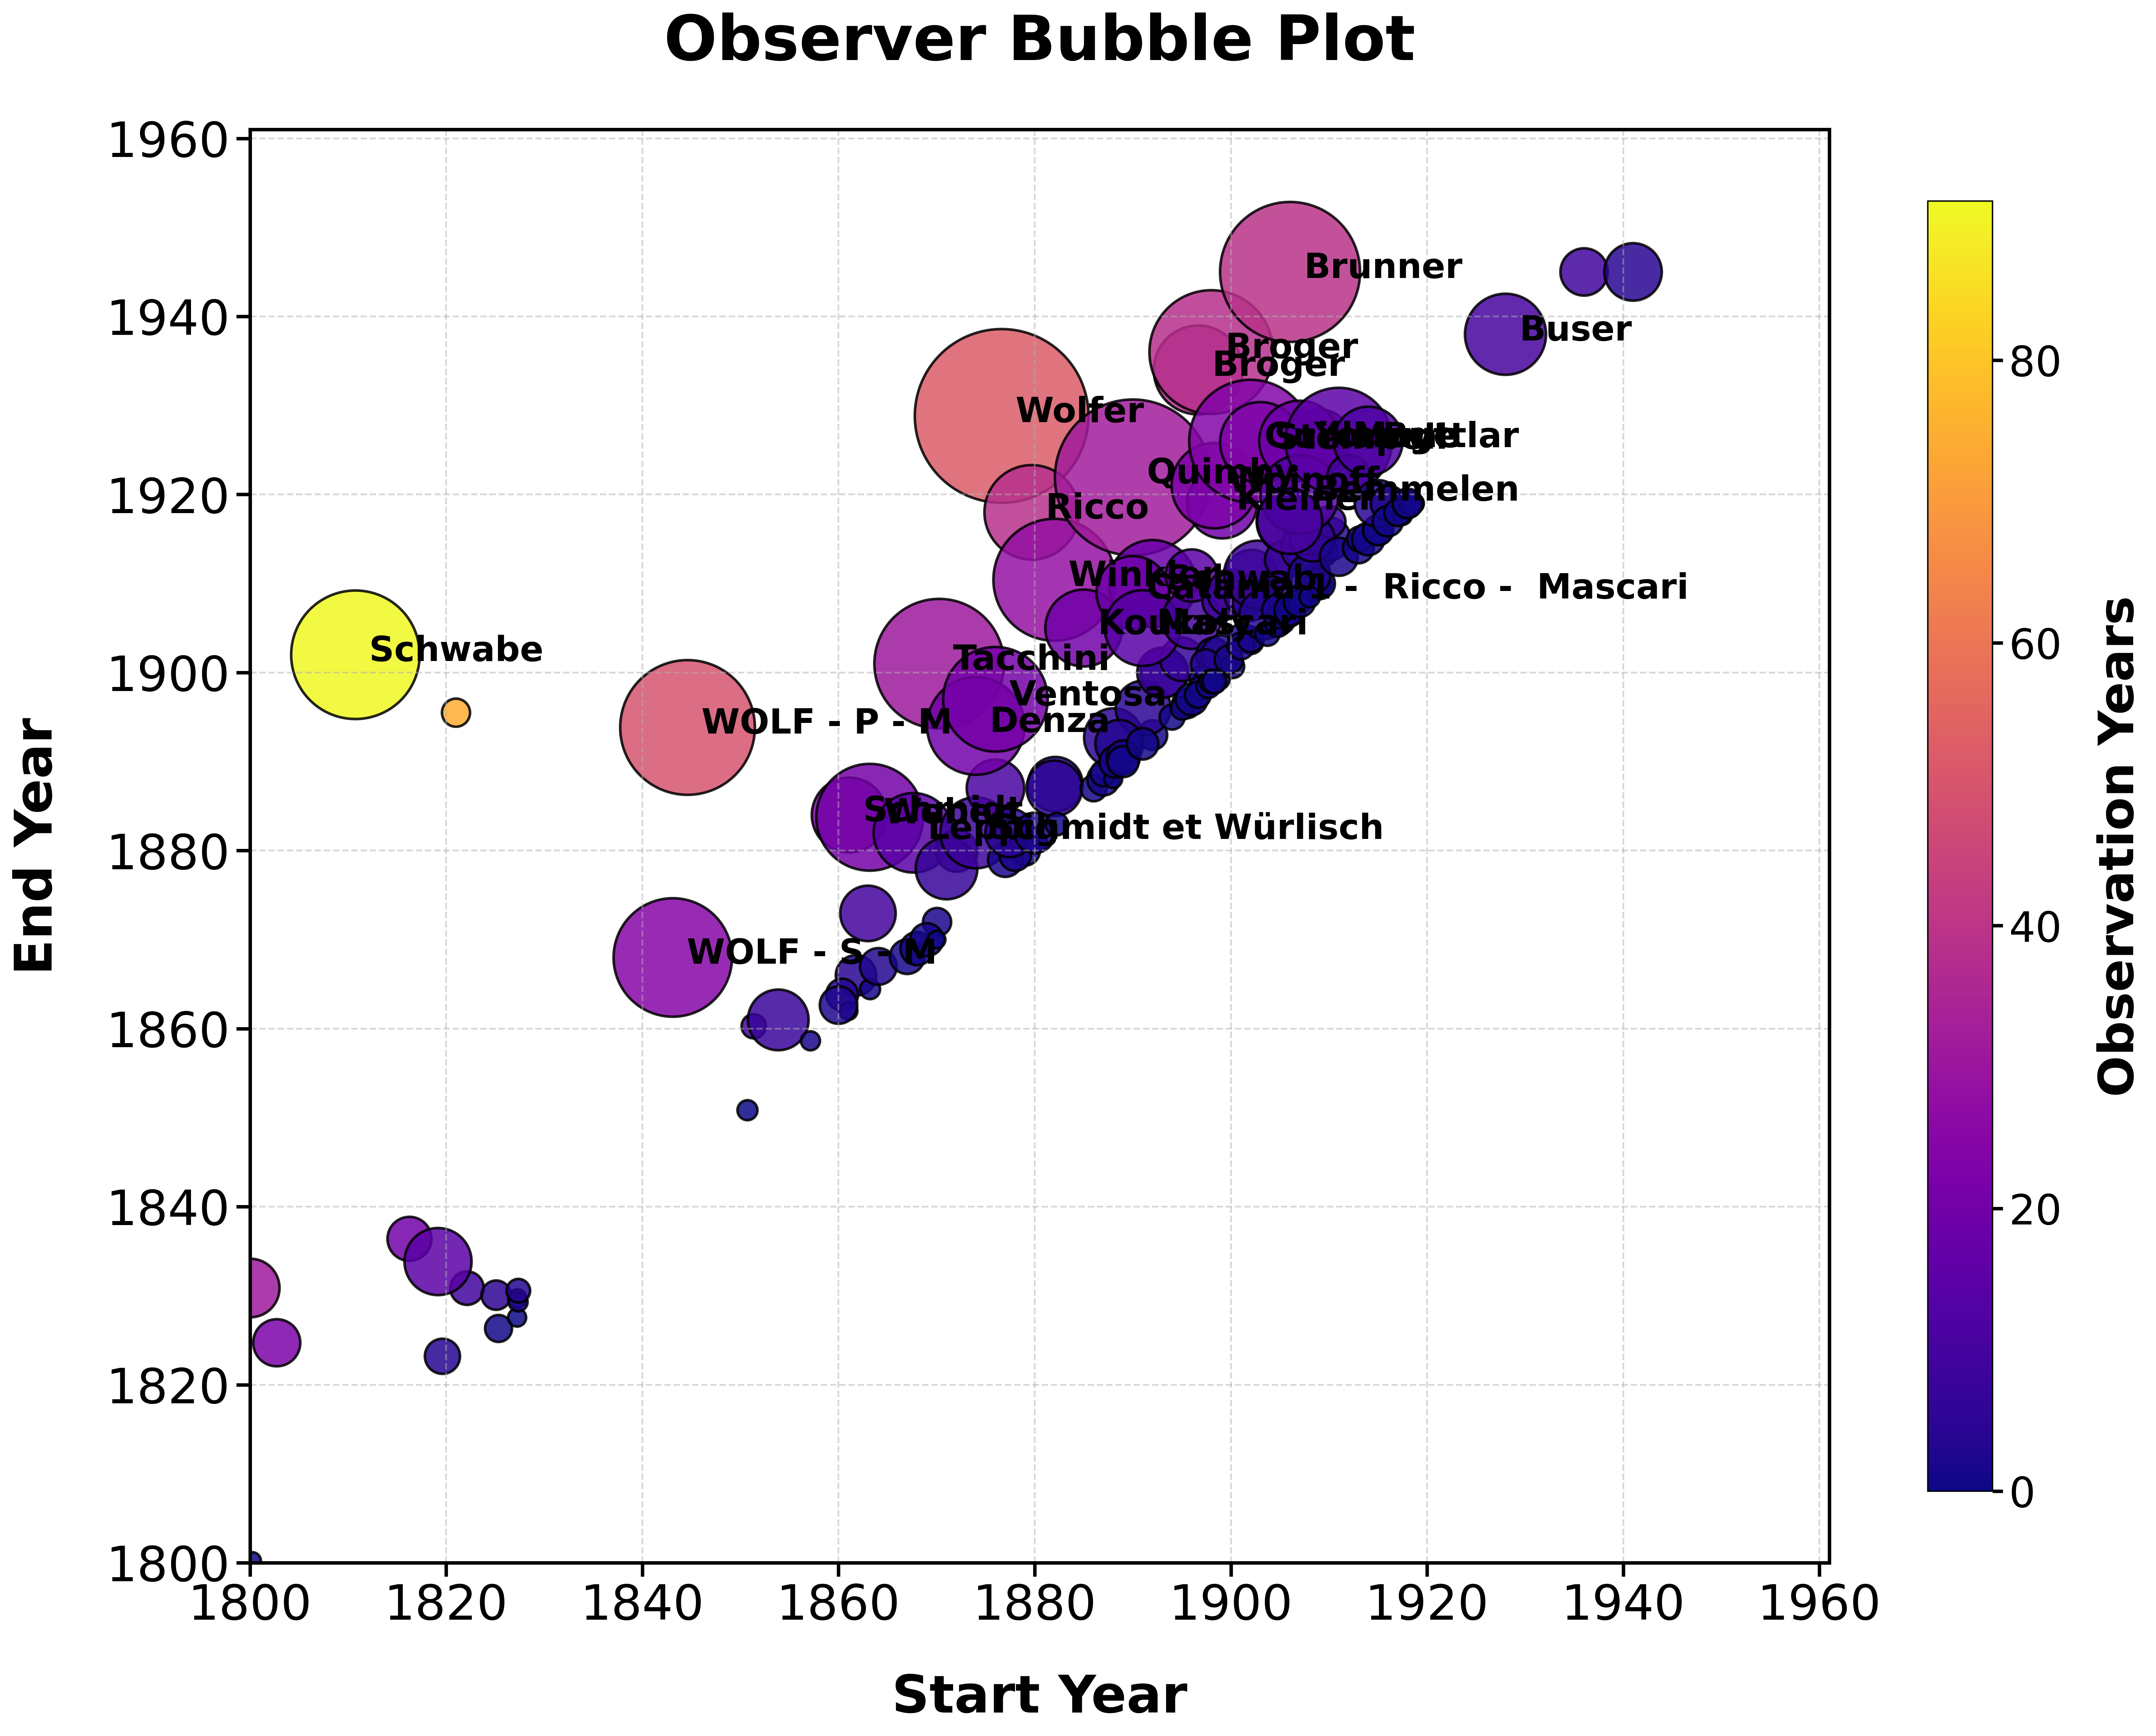
\includegraphics[width=\linewidth]{./figures/observer_bubbles_poster_v2.png}
    {\small (b) Observer coverage bubbles showing multi-century participation and overlaps}% that anchor cross-calibration.}
  \end{minipage}
  % \caption{\small Mittheilungen facsimile (a) and observer coverage overview (b) illustrating the documentation pipeline that links historical records to calibrated metadata.}
\end{figure}
\textbf{Z\"urich Tables (1945--1979)}\\
The Z\"urich Tables form the foundational record of daily sunspot number production at the Z\"urich Observatory between 1945 and 1979, detailing group and spot counts, the adopted Wolf number, and observing context.

\textbf{Current status}
\begin{itemize}
  \item Fully digitized for 1945--1979 with detailed metadata completed for 1945--1950.
  \item Ongoing quality control and observer metadata harmonisation to maintain traceability to the original ETH Z\"urich sources.
  \item Integrated within the consolidated FARSuN database, with citizen-science and VO/EPN-TAP access pathways in preparation.
\end{itemize}

\textbf{Next steps}
\begin{itemize}
  \item Complete metadata for later years, confirm 1980 holdings, and refine observer scaling (k-factors).
  \item Analyse the 1947 scale discontinuity and publish cleaned, validated releases linked with USET drawings.
  \item Deliver public access to the curated Z\"urich dataset to support reconstruction of ISN~V3.
\end{itemize}
\begin{figure}[t]
  \centering
  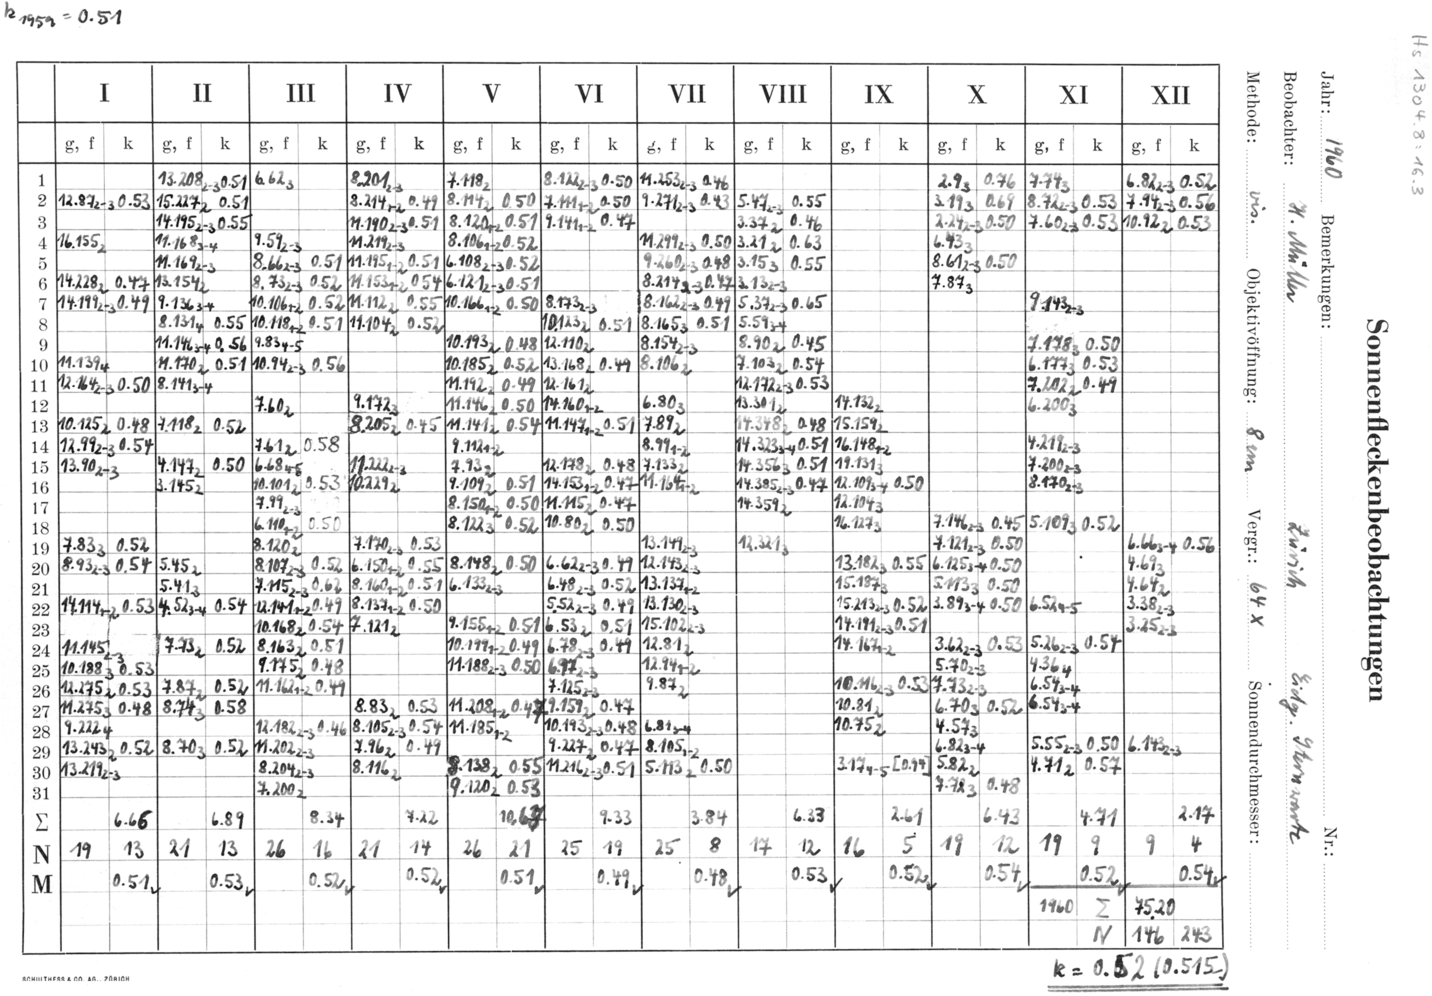
\includegraphics[width=0.85\linewidth]{./figures/zurich_tables.png}
  \caption{\small Facsimile of a typical handwritten yearly table from the complete 1945--1980 collection recovered in 2018--2019. Shown are H.~M\"uller's 1960 observations with group totals, spot counts, personal $k$ relative to Waldmeier, sky quality, monthly aggregates, and yearly averages, highlighting assistant-to-primary dispersion (here $k=0.52$ versus the 0.6 target).}
\end{figure}
\textbf{C.~H. Adams Sunspot Data — Present Status \& Future Work}\\
FARSuN has recovered 338 full-disk drawings and 1,056 daily entries (308 spot days, 748 spotless) from C.~H.~Adams (1819--1823), providing dense coverage with explicit spotless days that sharpen low-activity baselines for ISN~V3.

\textbf{Current work}
\begin{itemize}
  \item Quality-control passes to reconcile direct versus reflection methods and ensure consistent calibration.
  \item Cross-validation against \emph{Mittheilungen} and contemporaneous observers for contextual agreement.
  \item Orientation, dewarping, and standardisation of drawings to enable future positional and area extractions.
\end{itemize}
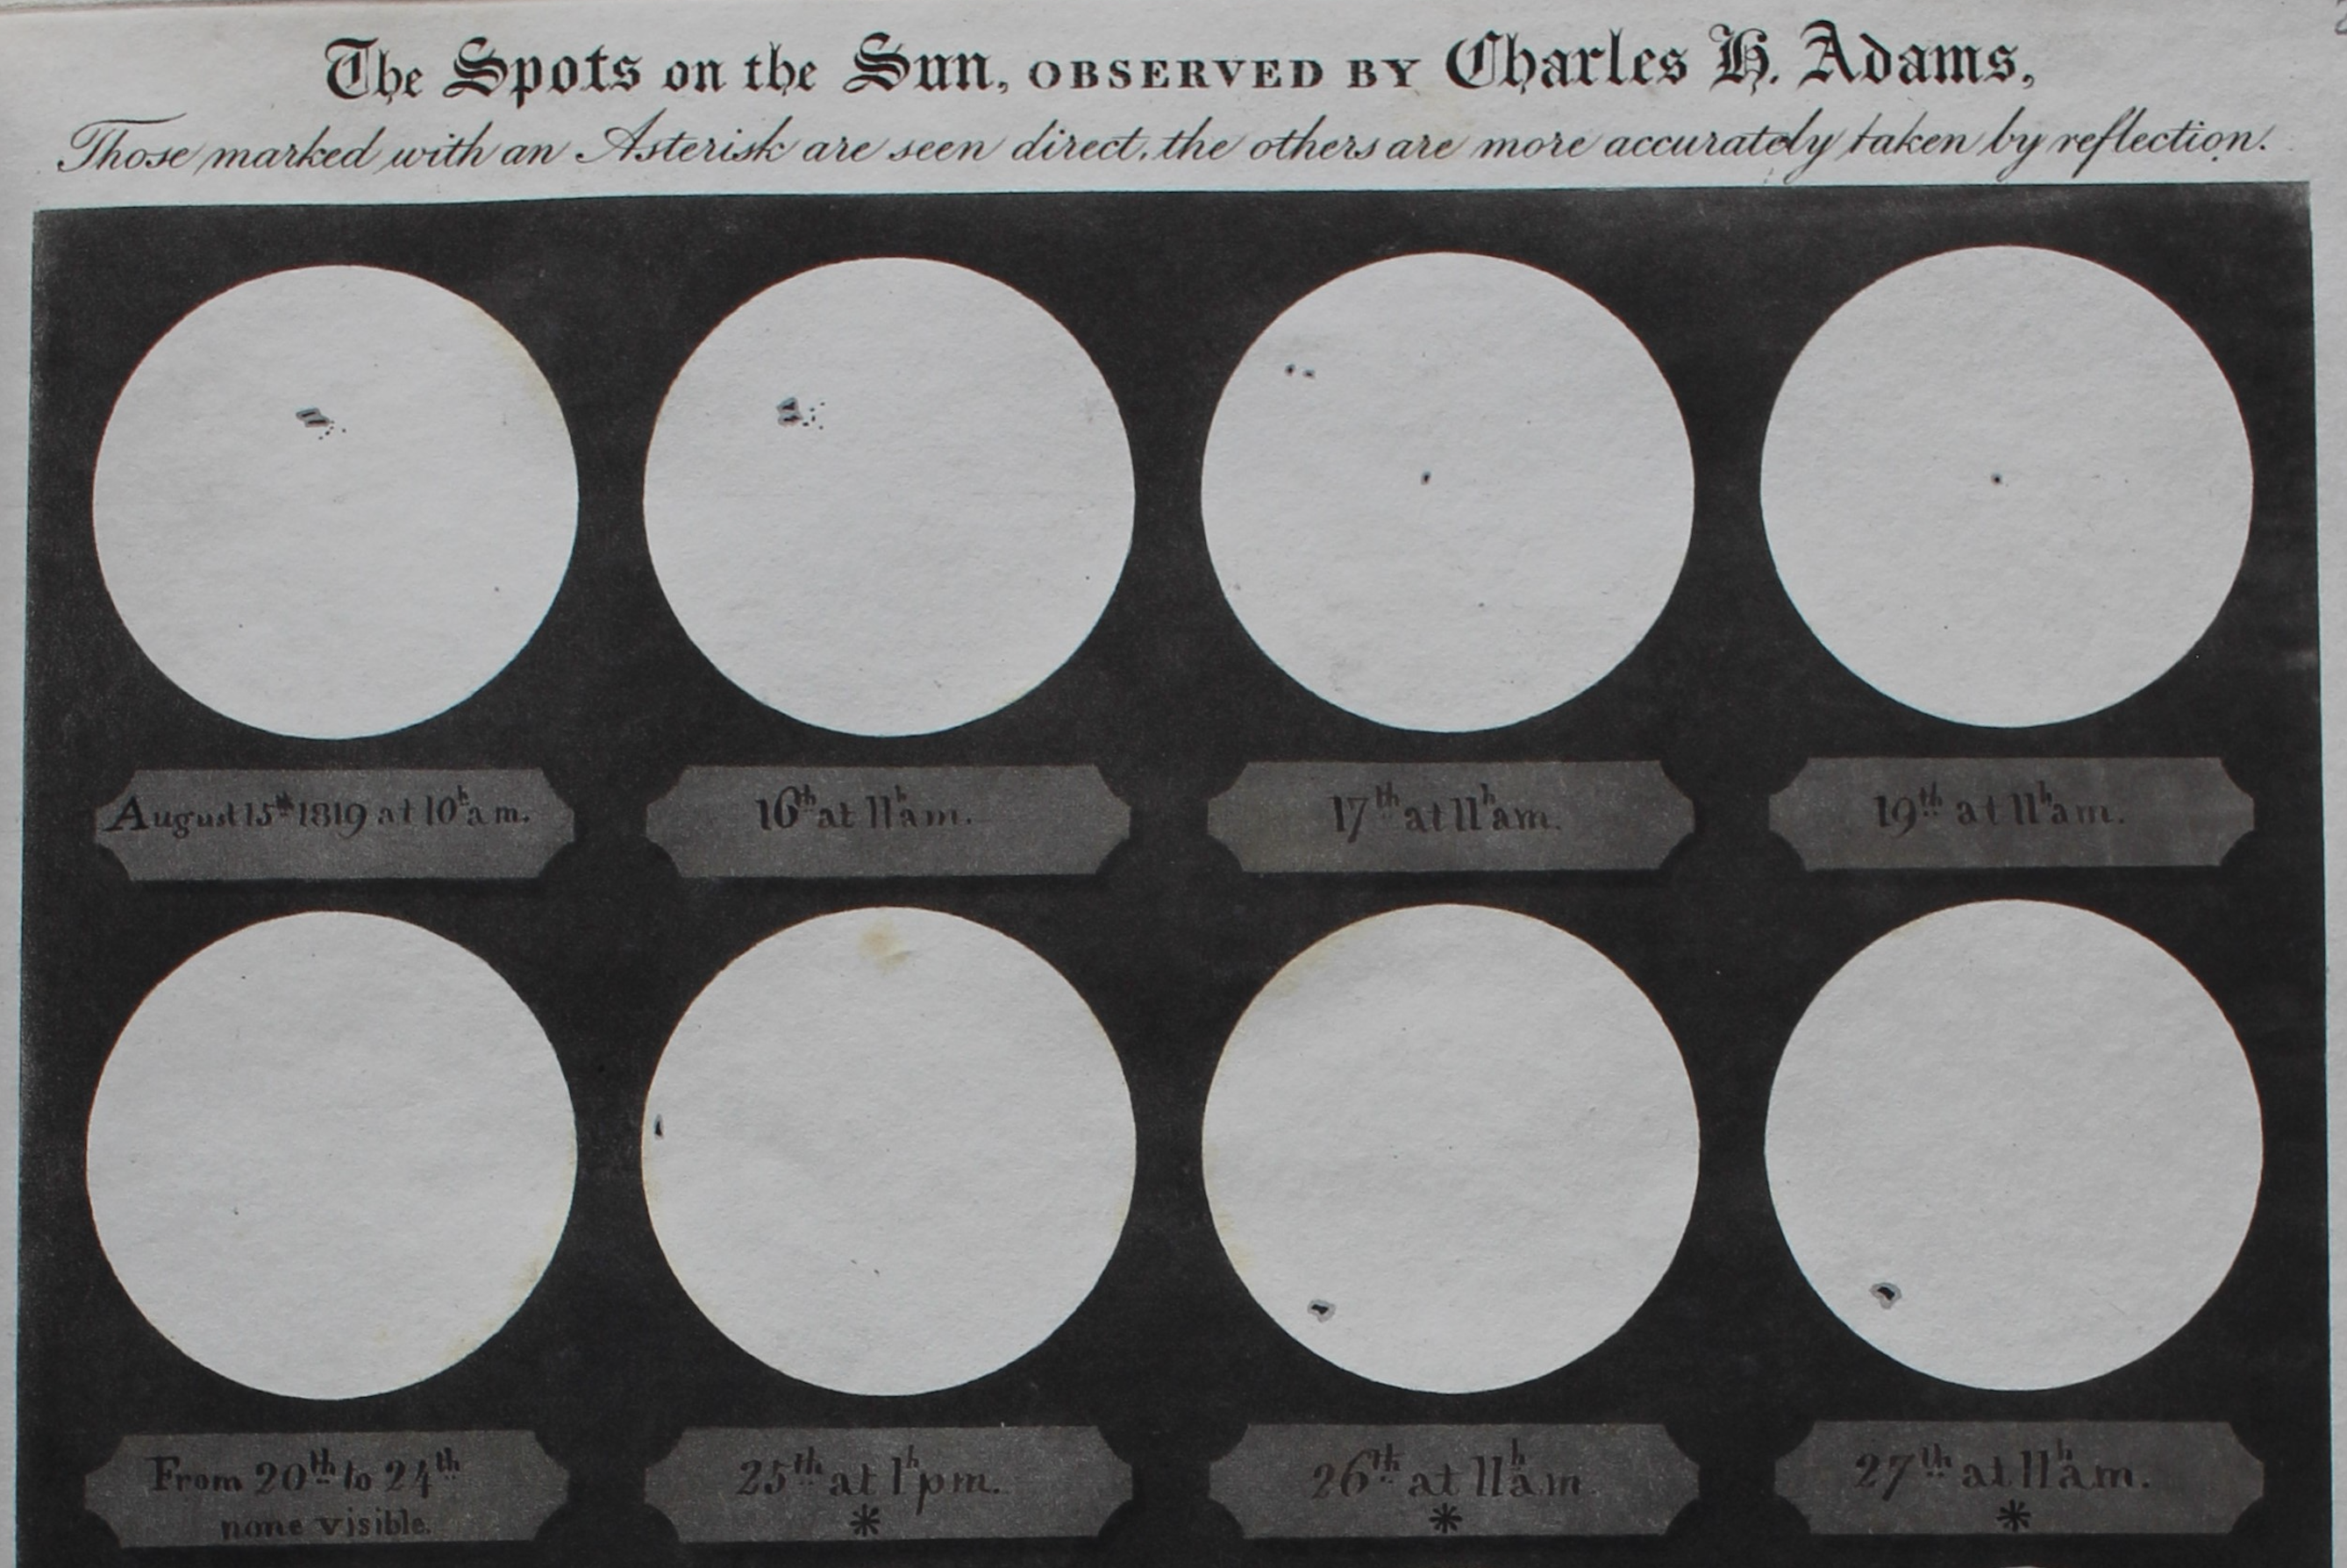
\includegraphics[width=\linewidth]{./figures/adams_example.png}
\end{tightblock}

\begin{tightblock}{Progress Highlights (Early 2025)}
\begin{itemize}
  \item Citizen-science ready interface blueprint finished; aligns with planned public transcription portal.
  \item Zürich production line blends Transkribus-assisted extraction with manual review to hit 2025 completion.
  \item Gruithuisen workflow pairs Kurrent script specialists with validation scripts to flag missing sun symbols.
  \item Adams drawings compared against \emph{Mittheilungen} daily records to benchmark spotless-day agreement.
\end{itemize}
\end{tightblock}

\begin{tightblock}{Observer Timeline}
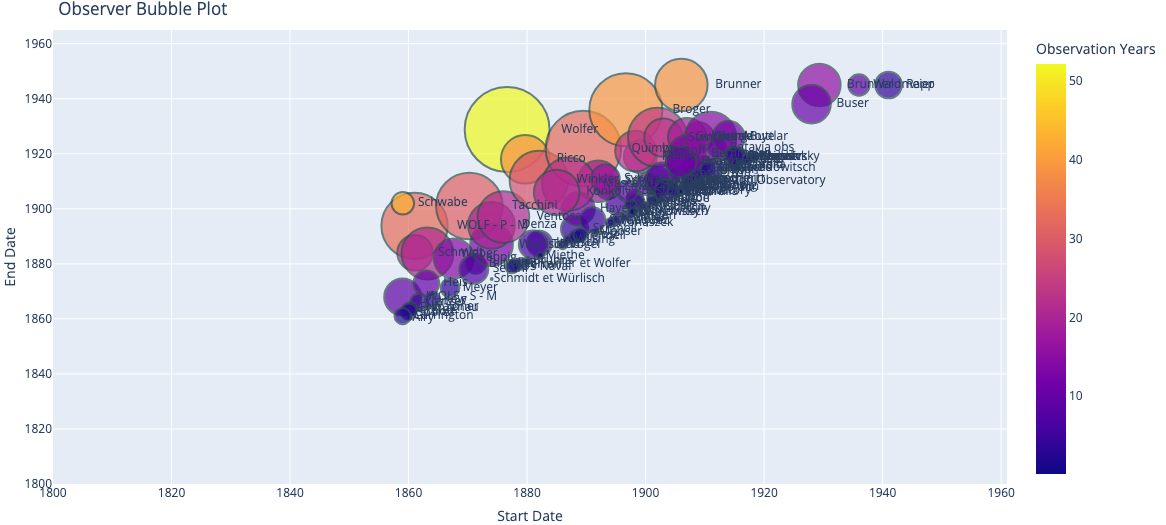
\includegraphics[width=\linewidth]{./figures/observers_bubble.png}
\scriptsize (Bubble size = total observations; color = years)
\end{tightblock}

\begin{tightblock}{Methods}
\begin{itemize}
  \item Dual-mode transcription: tailored Transkribus handwriting models plus manual keying for complex tables.
  \item Data hygiene: observer alias reconciliation, calendar conversions, and spot/group recount audits.
  \item Uncertainty modelling: propagate observer calibration curves and note spotless-day confidence flags.
  \item Automation: reproducible Python pipelines with checkpoints for citizen-science ingestion and review.
\end{itemize}
\end{tightblock}

\begin{tightblock}{Quality Gates}
\begin{itemize}
  \item Two-person verification for Adams and Gruithuisen counts before publishing derived indices.
  \item Cross-compare FARSuN transcriptions with Wolf's \emph{Mittheilungen} and modern SILSO indices for drift detection.
  \item Metadata harmonisation ensures unique observer IDs, instrument notes, and weather context survive downstream.
  \item Git-tracked pipelines and notebooks capture every transformation for audit and reuse.
\end{itemize}
\end{tightblock}
\end{column}

% -------- COLUMN 3 --------
\begin{column}{0.27\paperwidth}
\begin{tightblock}{Key Datasets}
\begin{tabular}{@{}p{0.33\linewidth}p{0.23\linewidth}p{0.38\linewidth}@{}}
\toprule
\textbf{Source} & \textbf{Period} & \textbf{Current Focus} \\ \midrule
\emph{Mittheilungen} & 1610--1945 & Fully digitized and integrated; observer statistics produced from 400+ years of entries. \\
Zürich Tables & 1945--1979 & 95\% of 2\,000+ tables digitized; metadata encoding for late-1970s observers underway. \\
Gruithuisen Manuscripts & 1817--1849 & 100\% digitized; Extraction using transkribus like models + dual QC for group/spot counts underway. \\
C. H. Adams Drawings & 1819--1823 & 338 sketches extracted (1\,056 entries); spotless days cross-checked against Wolf series. \\
Augustin Stark Ledgers & 1813--1835 & Normalizing tabular layouts; linking weather annotations to group counts. \\
Rost Journals & 18th--19th c. &  \\
\bottomrule
\end{tabular}
\end{tightblock}

\begin{tightblock}{From Raw to ISN V3}
\begin{enumerate}
  \item Curate daily counts with provenance-rich metadata (observer, instrument, weather context).
  \item Solve observer response functions to align group/spot scales across centuries.
  \item Aggregate to monthly, yearly, and hemispheric indices with propagated uncertainties.
  \item Benchmark against ISN~V2 and satellite-era proxies to validate drift corrections.
\end{enumerate}
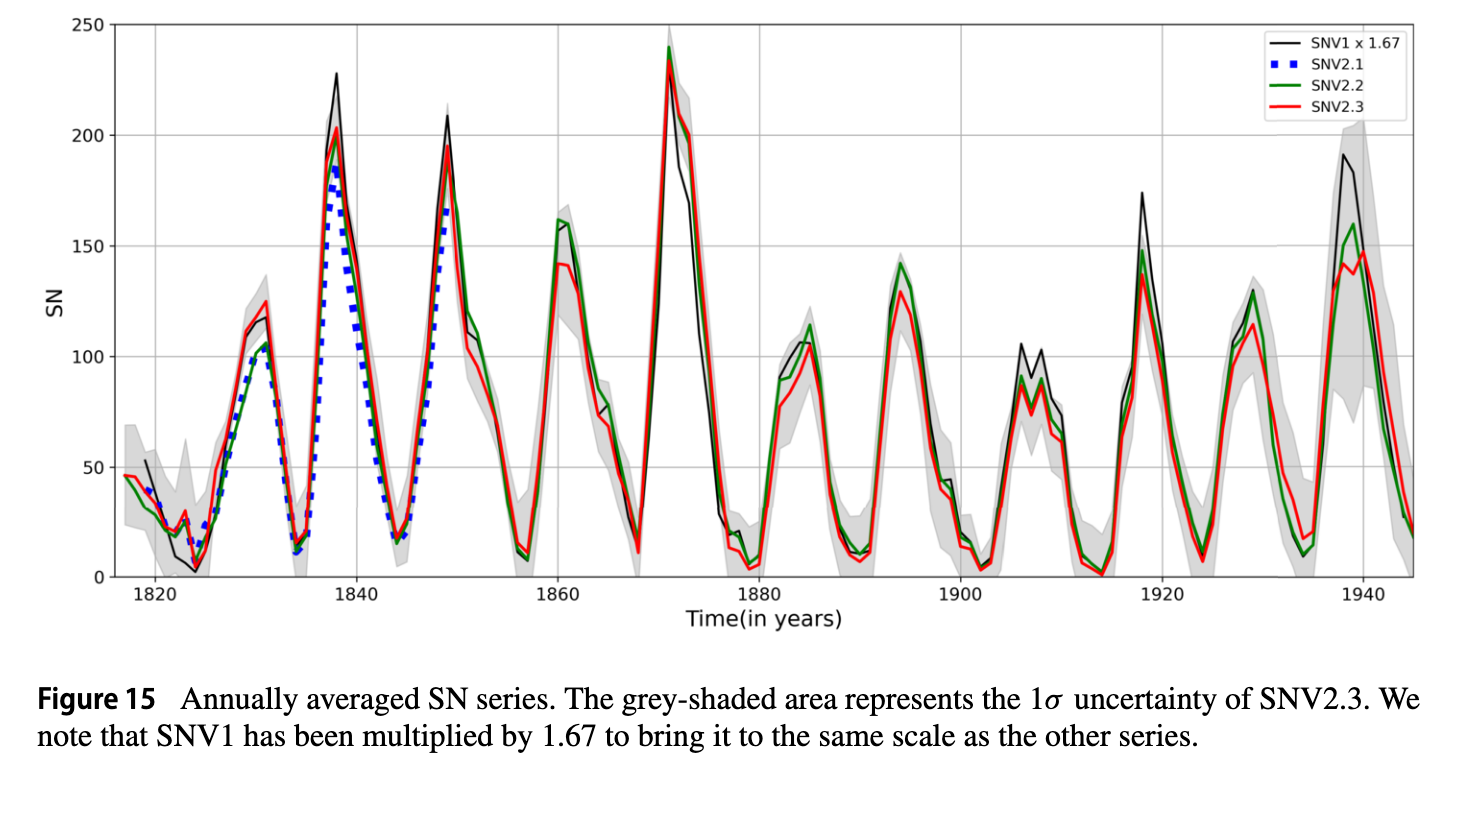
\includegraphics[width=0.9\linewidth]{./figures/comparison_panel.png}
\end{tightblock}

\begin{tightblock}{Challenges}
\begin{itemize}
  \item Deciphering \emph{Kurrent} manuscripts and annotating non-solar notes without losing context.
  \item Harmonising heterogeneous formats (drawings, tabular ledgers, weather marginalia).
  \item Quantifying observer bias and spotless-day reporting habits over centuries.
  \item Maintaining end-to-end provenance from scanned folio to released data product.
\end{itemize}
\end{tightblock}

\begin{tightblock}{Space Climate Impact}
\begin{minipage}[t]{0.48\linewidth}
  \callout{Citizen science}{Interactive portal mobilises volunteers to transcribe \emph{Kurrent} manuscripts and sustain STEM outreach.}
\end{minipage}\hfill
\begin{minipage}[t]{0.48\linewidth}
  \callout{Forecasting}{Bias-free ISN~V3 improves solar cycle prediction skill and operational space weather baselines.}
\end{minipage}\\[0.6em]
\begin{minipage}[t]{0.48\linewidth}
  \callout{Climate links}{Validated historical forcing refines long-term climate models and Earth radiation budget studies.}
\end{minipage}\hfill
\begin{minipage}[t]{0.48\linewidth}
  \callout{Open science}{FAIR-compliant releases with APIs and uncertainty bundles accelerate community reuse.}
\end{minipage}
\end{tightblock}

\begin{tightblock}{Outlook}
\begin{itemize}
  \item Launch citizen-science transcription portal with tailored training sets.
  \item Publish ISN~V3 release notes with uncertainty budget and API endpoints.
  \item Expand collaborations (Nagoya, UCLouvain, ROB) for cross-validation and joint publications.
\end{itemize}
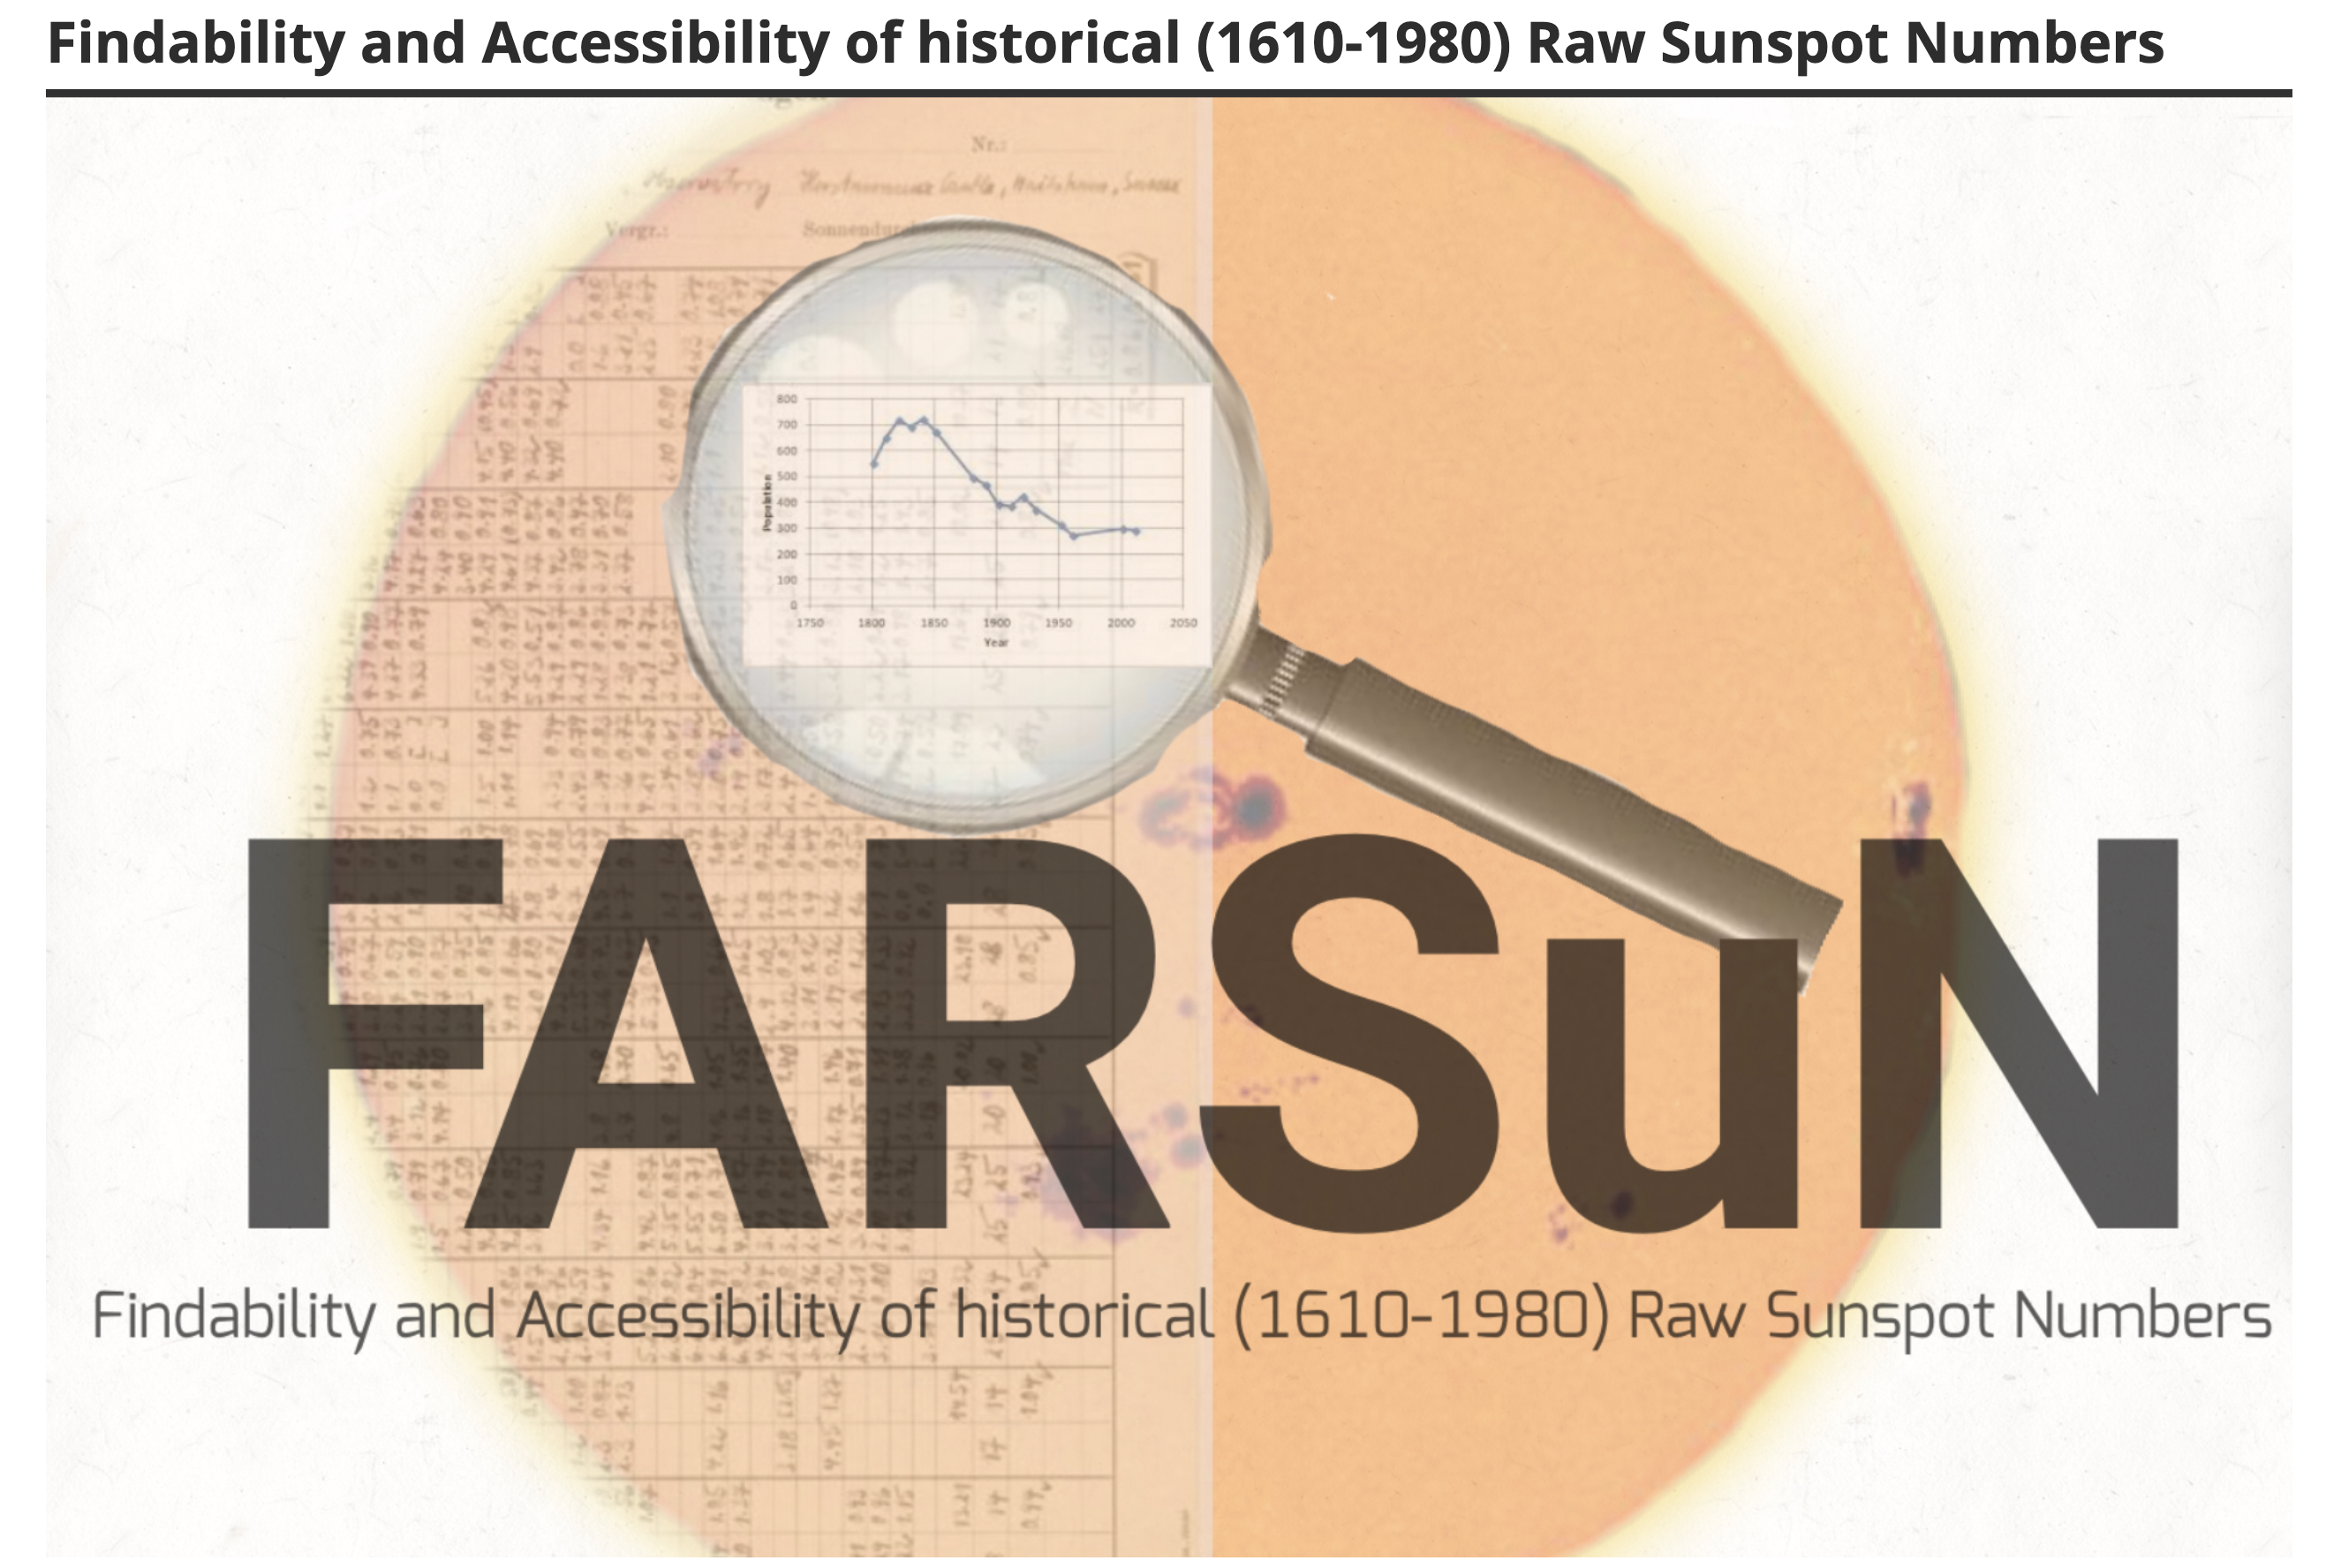
\includegraphics[width=0.8\linewidth]{./figures/ack_.png}
\end{tightblock}

\begin{tightblock}{References}
{\footnotesize \bibliography{articles}}
\end{tightblock}
\end{column}

\end{columns}
\end{frame}
\end{document}
